%--------------------------------------------
% Chapter: DEVELOPMENT ENVIRONMENT
%--------------------------------------------
\chapter{Development Environment (Virtual Machine Image and Native Machine)}
\label{sec:sec-VM}

This project uses the VMWare player of the company VMWare \footnote{https://my.vmware.com/de/web/vmware/free\#desktop\_end\_user\_computing/vmware\_player/7\_0}. This gives the ability that no dependency to a special operating system exists. It can run on any system like mac, windows or linux. A pre defined Image for the VMWare player can be found in the SVN repository folder \texttt{/sys/VM/}.
The native machine is based on 14.04 AMD64 Ubuntu.
If you have native machine and running the program there, then please directly skip to 
the section \textbf{Toolchain}

\begin{figure}[H]
	\centering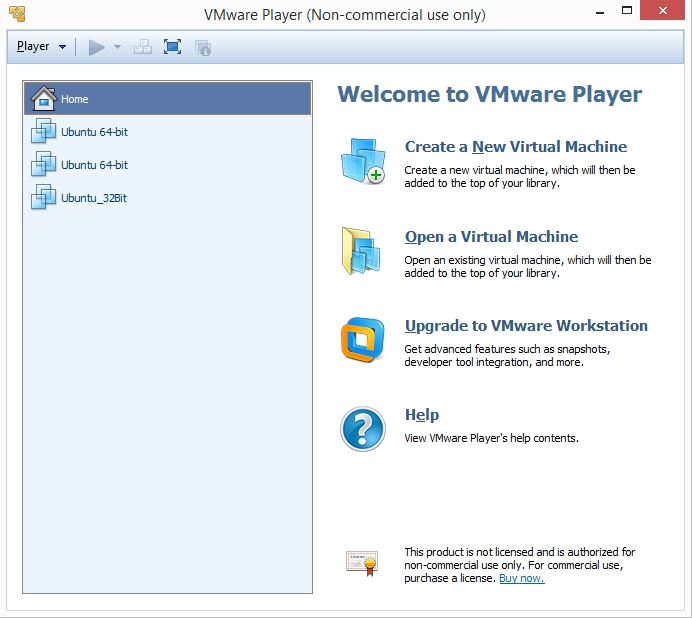
\includegraphics[width=0.5\textwidth]{fig/Dev_Concept/VMPlayer.jpg}
	\caption{VMWare Player}
	\label{fig:VMPlayer}
\end{figure}

\section{Ubuntu}
\label{subsec:sec-Ub}

Here the current Ubuntu 14.10 which is installed with the help of the VMWare player is used. For programming the software eclipse is taken. First the current image of Ubuntu needs to be downloaded:
\begin{lstlisting}
http://www.ubuntu.com/download
\end{lstlisting}
Figure \ref{fig:Ub1} shows the the window of the VMWare player directly after starting. To add a new virtual machine a click on 'Create a New Virtual Machine' has to be made.

\begin{figure}[H]
	\centering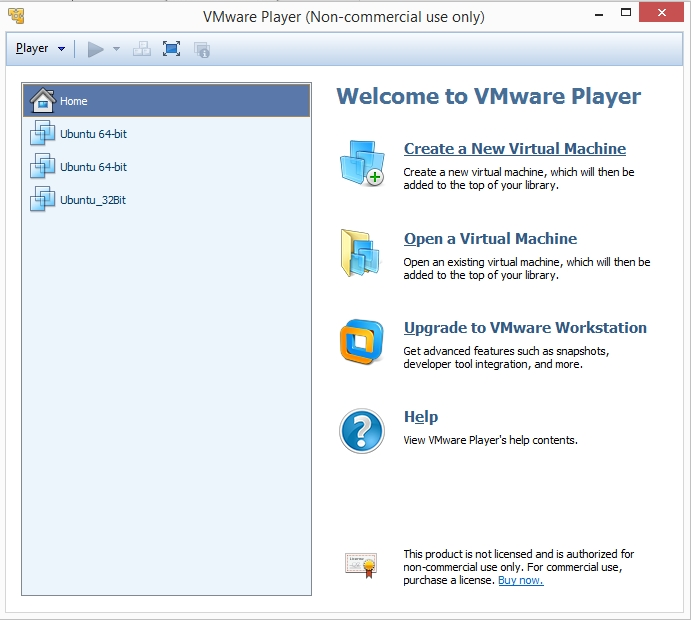
\includegraphics[width=0.4\textwidth]{fig/Dev_Concept/Ub1.jpg}
	\caption{Installing Ubuntu - Step 1: Create new virtual machine}
	\label{fig:Ub1}
\end{figure}

Then under the 'Installer disc image file (iso)', the path to the before downloaded ISO-file needs to be set like in the figure \ref{fig:Ub2}.

\begin{figure}[H]
	\centering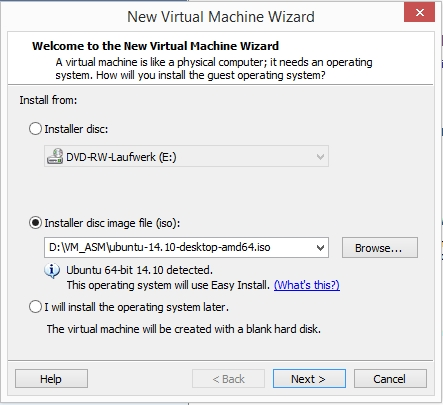
\includegraphics[width=0.4\textwidth]{fig/Dev_Concept/Ub2.jpg}
	\caption{Installing Ubuntu - Step 2: Installer ISO-file}
	\label{fig:Ub2}
\end{figure}

Figure \ref{fig:Ub3} shows the next step. A full name, a user and a password is set. In this project 'user' with password 'user' is used.

\begin{figure}[H]
	\centering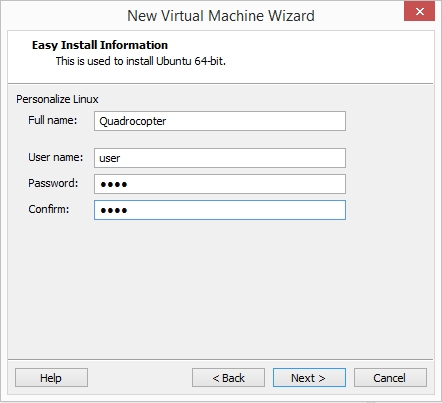
\includegraphics[width=0.5\textwidth]{fig/Dev_Concept/Ub3.jpg}
	\caption{Installing Ubuntu - Step 3: Setting up a generic user}
	\label{fig:Ub3}
\end{figure}

Then a name for the virtual machine and the location, where the virtual machine is stored is chosen. See figure \ref{fig:Ub4}.

\begin{figure}[H]
	\centering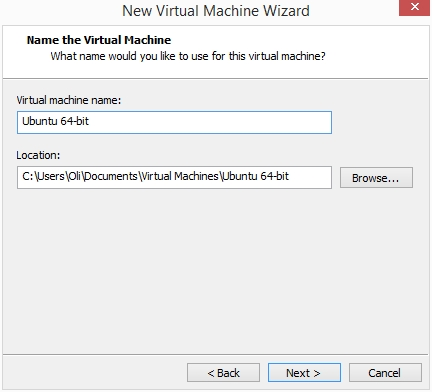
\includegraphics[width=0.5\textwidth]{fig/Dev_Concept/Ub4.jpg}
	\caption{Installing Ubuntu - Step 4: Name of virtual machine}
	\label{fig:Ub4}
\end{figure}

The following figures \ref{fig:Ub5} and \ref{fig:Ub6} show the option for the size and the splitting and finally a summary.

\begin{figure}[H]
	\centering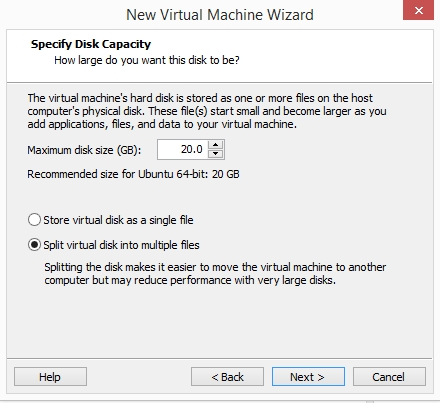
\includegraphics[width=0.5\textwidth]{fig/Dev_Concept/Ub5.jpg}
	\caption{Installing Ubuntu - Step 5: Choosing virtual disk size}
	\label{fig:Ub5}
\end{figure}

\begin{figure}[H]
	\centering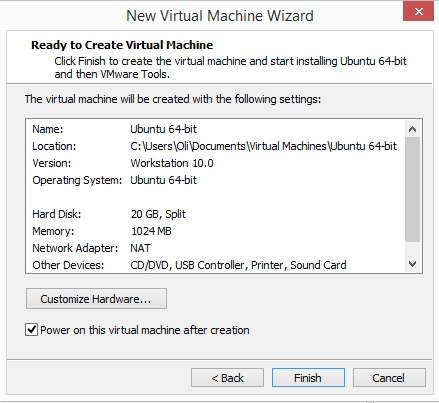
\includegraphics[width=0.5\textwidth]{fig/Dev_Concept/Ub6.jpg}
	\caption{Installing Ubuntu - Step 6: Finalize virtual machine}
	\label{fig:Ub6}
\end{figure}

Then VMWare tools wants to be installed. This tool is needed for example to enable dynamic rescaling of the Desktop of Ubuntu within the VMWare player, so it should be installed. See figure \ref{fig:Ub7}.

\begin{figure}[H]
	\centering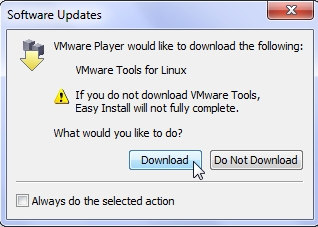
\includegraphics[width=0.5\textwidth]{fig/Dev_Concept/Ub7.jpg}
	\caption{Installing Ubuntu - Step 7: Installation of VMWare Tools}
	\label{fig:Ub7}
\end{figure}

Finally the login window of Ubuntu (figure \ref{fig:Ub9}).

\begin{figure}[H]
	\centering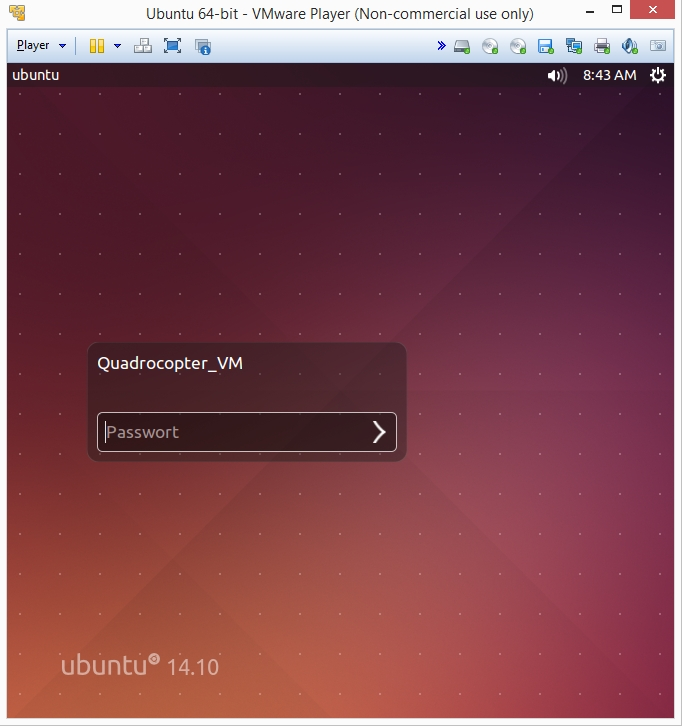
\includegraphics[width=0.5\textwidth]{fig/Dev_Concept/Ub9.jpg}
	\caption{Installing Ubuntu - Step 8: Ubuntu's system login}
	\label{fig:Ub9}
\end{figure}

Remark:\\
If the rescaling later on will not work, then after the start and login into Ubuntu, the following command needs to run in the terminal window:
\begin{lstlisting}[language=bash,otherkeywords={sudo,tar,touch,gedit,cp,apt-get,mkdir}]
sudo apt-get install open-vm-tools-desktop
\end{lstlisting}


\section{Toolchain}
\label{subsec:sec-TC}

A Toolchain enables compilation on the fast development computer instead on the Raspberry Pi. This is called cross compiling. To make it possible, following commands have to be called in the Ubuntu operating system which is running in the virtual machine. This description is based on the blog entry from Halherta \footnote{http://hertaville.com/2012/09/28/development-environment-raspberry-pi-cross-compiler/}.\\
First the cross compiling toolchain will be downloaded and set up. The following commands will be called in a terminal window.\\
The following command downloads the native build tools and the GIT tool which will be used to download the cross compiling toolchain.
\begin{lstlisting}[language=bash,otherkeywords={sudo,tar,touch,gedit,cp,apt-get,mkdir}]
sudo apt-get install build-essential git
\end{lstlisting}
Next a directory is created and then the directory is opened.
\begin{lstlisting}[language=bash,otherkeywords={sudo,tar,touch,gedit,cp,apt-get,mkdir}]
mkdir rpi
cd rpi
git clone git://github.com/raspberrypi/tools.git
\end{lstlisting}
The last command downloads the official cross compiling Toolchain. 
In the folder \newline/home/user/rpi/tools/arm-bcm2708 are now four different folders stored which contain different toolchains.
\begin{lstlisting}[language=bash]
 arm-bcm2708-linux-gnueabi
 arm-bcm2708hardfp-linux-gnueabi
 gcc-linaro-arm-linux-gnueabihf-raspbian
 gcc-linaro-arm-linux-gnueabihf-raspbian-x64
\end{lstlisting}
Due to the reason that the used Ubuntu is a 64 bit OS the fourth toolchain has to be used.
To enable compilation also directly from the command line, the path to the Toolchain has to be added in the PATH variable of the Ubuntu system. To do so, the following actions need to be done.

\begin{lstlisting}[language=bash,otherkeywords={sudo,tar,touch,gedit,cp,apt-get,mkdir},escapechar=|]
cd ~/
nano .bashrc
export PATH=$PATH:$HOME/rpi/tools/arm-bcm2708/|\\|gcc-linaro-arm-linux-gnueabihf-raspbian-x64/bin
source .bashrc
\end{lstlisting}
The last command updats the PATH variable.\\
If all actions are successfully done, it can be proved by:
\begin{lstlisting}[language=bash]
arm-linux-gnueabihf-gcc -v
\end{lstlisting}
If all works fine the terminal window should show following output.

\begin{figure}[H]
	\centering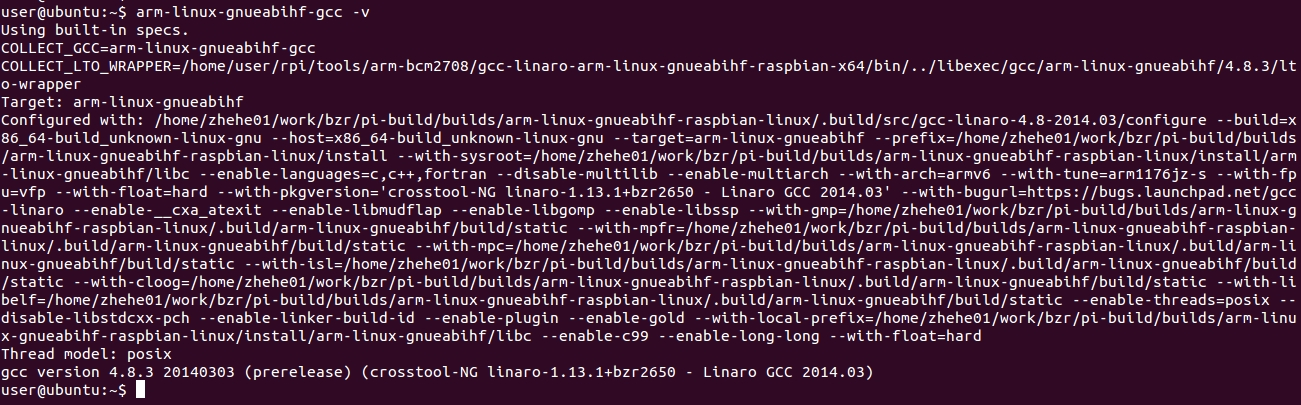
\includegraphics[width=1\textwidth]{fig/Dev_Concept/Cross_compile_success.jpg}
	\caption{Prove of successfull working Toolchain}
	\label{fig:Cross_compile_success}
\end{figure}

\section{Eclipse}
\label{subsec:subsec-Eclipse-header}

\subsection{Installation of Eclipse Luna}
\label{subsec:subsec-Eclipse}

Next, the current 64 Bit Eclipse IDE for C/C++ Developers, is downloaded from the webpage of eclipse within the Ubuntu system:
\begin{lstlisting}
https://www.eclipse.org/downloads/?osType=linux
\end{lstlisting}

First the current Java runtime environment is installed.
\begin{lstlisting}[language=bash,otherkeywords={sudo,tar,touch,gedit,cp,apt-get,mkdir}]
sudo apt-get install openjdk-7-jre
\end{lstlisting}
Then the before downloaded eclipse is extracted and stored to /opt
\begin{lstlisting}[language=bash,otherkeywords={sudo,tar,touch,gedit,apt-get,mkdir}]
sudo tar -xvzf eclipse-cpp-luna-SR2-linux-gtk-x86_64 -C /opt/
\end{lstlisting}
In order to access the most recent eclipse, a custom desktop link has to be created and edited. 
\begin{lstlisting}[language=bash,otherkeywords={sudo,tar,touch,gedit,cp,apt-get,mkdir}]
sudo touch /usr/share/applications/eclipse-recent.desktop;
sudo gedit /usr/share/applications/eclipse-recent.desktop &
\end{lstlisting}
An editor will open after executing the above shown lines. Paste the following lines in order to create a valid Ubuntu desktop launcher:
\begin{lstlisting}
[Desktop Entry]
Type=Application
Name=Eclipse Luna
Comment=Eclipse Integrated Development Environment
Icon=/opt/eclipse/icon.xpm
Exec=/opt/eclipse/eclipse
Terminal=false
Categories=Development;IDE;Java;
\end{lstlisting}

Optionally, a starter icon can be put to the desktop of Ubuntu by copying the above created Ubuntu desktop launcher:
\begin{lstlisting}[language=bash,otherkeywords={sudo,cp,apt-get,mkdir}]
sudo cp /usr/share/applications/eclipse-recent.desktop ~/Desktop/
\end{lstlisting}

\subsection{Remote Debugging}
\label{subsubsec:subsubsec-RD}

Enabling remote debugging is really helpfull when a written program has not the  expected behaviour. To enable remote debugging, some configurations in the Debug Configurations need to be done. This window can be found under 'Run/Debug Configurations...'
In the starting window a click with the left mousebutton on 'C/C++ Remote Application' on the left part of the window needs to be done. Then click on 'New'. See figure \ref{fig:Debug1}.

\begin{figure}[H]
	\centering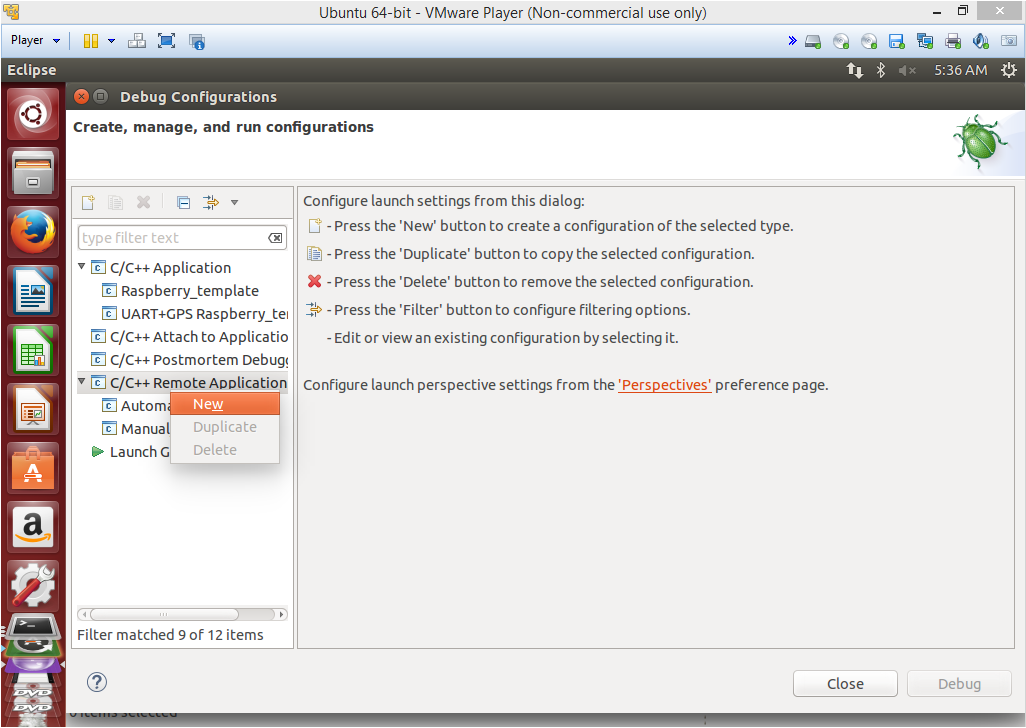
\includegraphics[width=0.7\textwidth]{fig/Dev_Concept/Debug1}
	\caption{Making new Debug Configuration}
	\label{fig:Debug1}
\end{figure}

In the appearing window write down first the Name 'Automatic\_Debug' and then in the tab 'Main' (see figure \ref{fig:Debug2}) write down the name of the project in the textfield 'Project:' and in 'C/C++ Application:' the executable, the binary file, which is in the Debug folder of the project. Under 'Build configuration' 'Use Active' and the radio button 'Enable auto build' has to be activated. When clicking under 'Connection:' on 'New...' a new window, like in figure \ref{fig:Debug3} appears. Here 'SSH only' and 'Next>' needs to be clicked. After that, in the next automatically popped up window all what needs to be written down can be seen in figure \ref{fig:Debug4}, and then it has to be confirmed by clicking on 'OK'. Last but not least there needs to be set a Folder which can be a existing or a new one in 'Remote Absolute File Path for C/C++ Application:' and under 'Commands to execute before application' the commands
\begin{lstlisting}[language=bash]
sudo -i
chmod +x Raspberry_Template
\end{lstlisting}
have to be included. Last make sure that in the lower area of the window 'Using GDB (DSF) Automatic Remote Debugging Launcher' is active.

\begin{figure}[H]
	\centering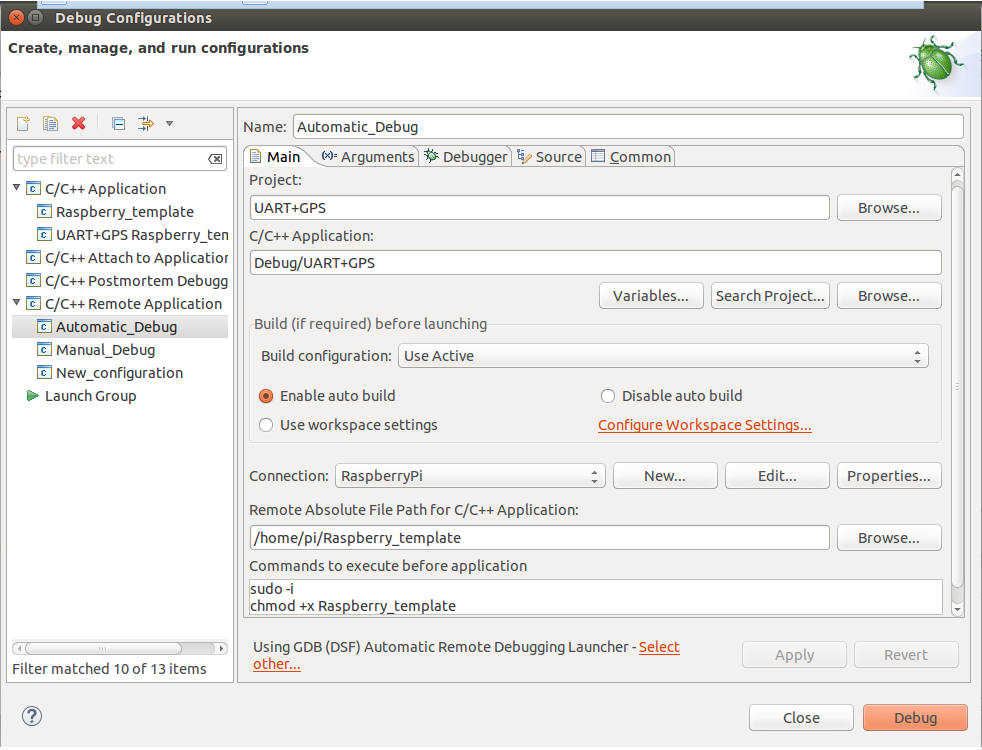
\includegraphics[width=0.9\textwidth]{fig/Dev_Concept/Debug2}
	\caption{Debug Configuration Window - Main tab}
	\label{fig:Debug2}
\end{figure}

\begin{figure}[H]
	\centering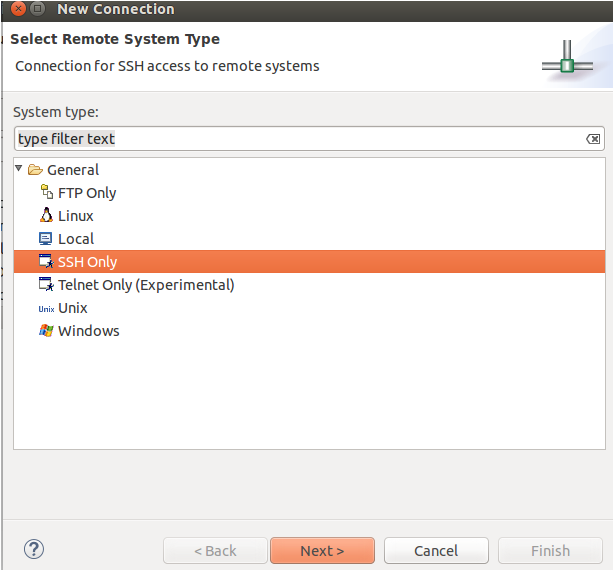
\includegraphics[width=0.5\textwidth]{fig/Dev_Concept/Debug3}
	\caption{Creating new connection 1}
	\label{fig:Debug3}
\end{figure}

\begin{figure}[H]
	\centering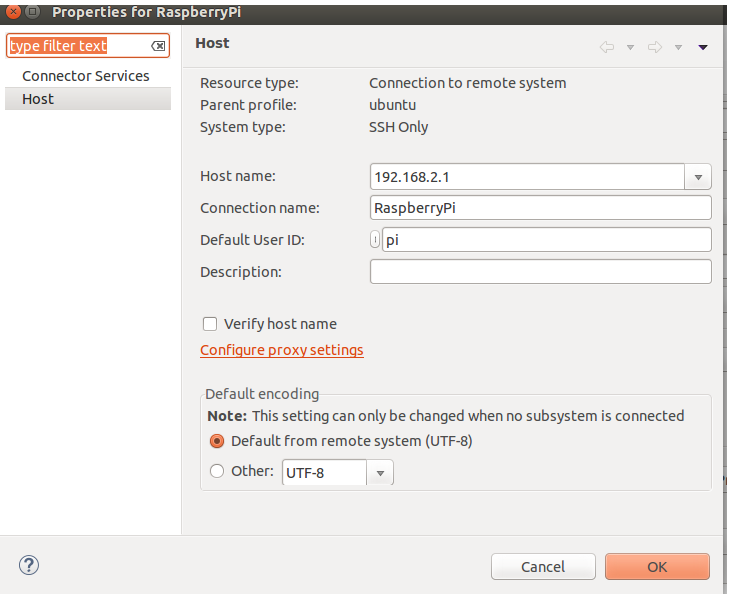
\includegraphics[width=0.7\textwidth]{fig/Dev_Concept/Debug4}
	\caption{Creating new connection 2}
	\label{fig:Debug4}
\end{figure}

\begin{figure}[H]
	\centering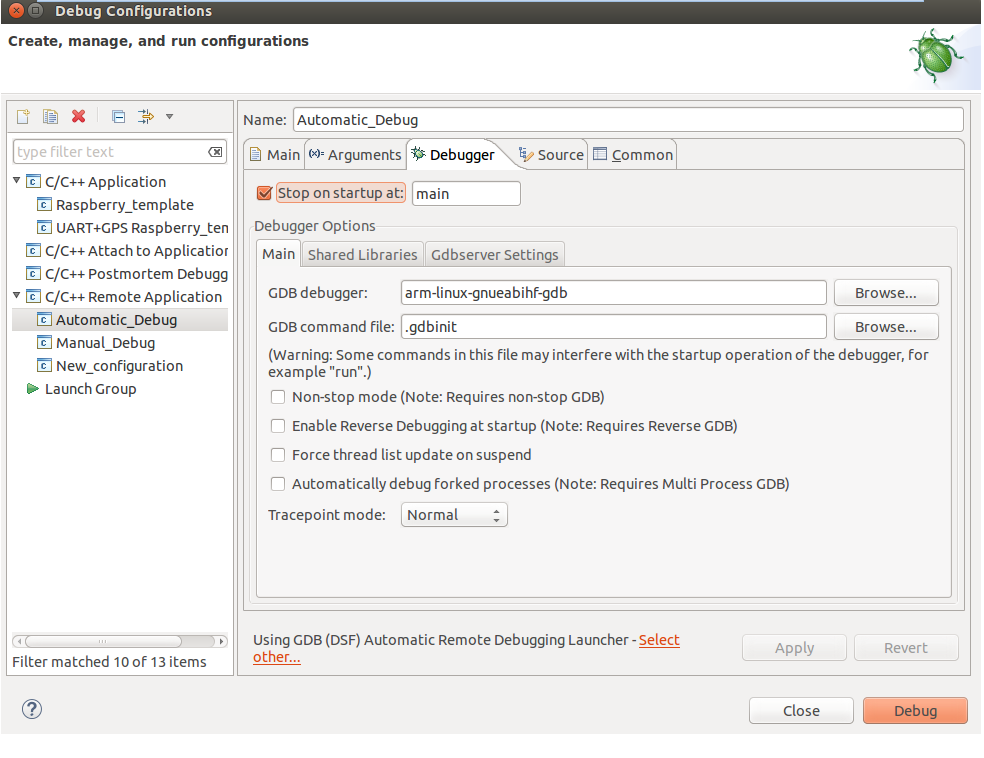
\includegraphics[width=0.9\textwidth]{fig/Dev_Concept/Debug6}
	\caption{Debug Configuration Window - Debugger tab}
	\label{fig:Debug6}
\end{figure}
After this is finished, in the Debugger tab, there needs in the 'GDB debugger' textfield 'arm-linux-gnueabihf-gdb' written down. This ensures that the ARM toolchain connects to the GDB server on the Raspberry (See figure \ref{fig:Debug6}).

\begin{figure}[H]
	\centering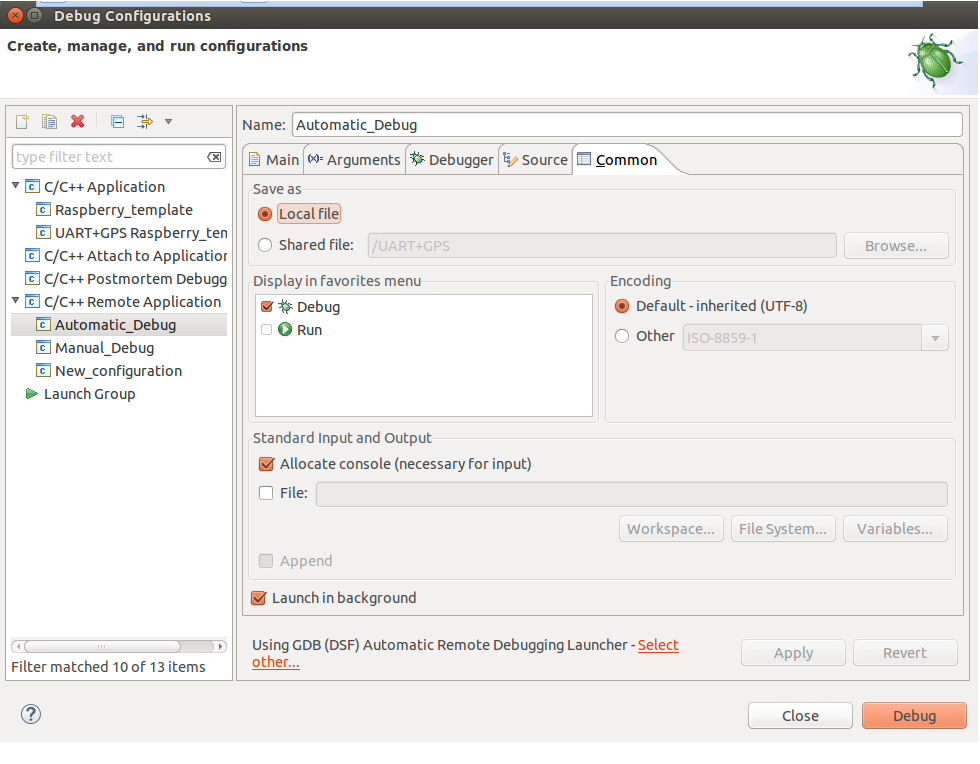
\includegraphics[width=0.9\textwidth]{fig/Dev_Concept/Debug7}
	\caption{Debug Configuration Window - Common tab}
	\label{fig:Debug7}
\end{figure}

Then in the 'Common' tab in 'Display in favorites menu' the 'Debug' checkbox needs to be activated. After that the window can be closed. Now all necessary actions are done and an existing project can be by debugged by clicking on the small arrow beneath the the small bug in the menu bar. Here the before saved Configuration (Automatic\_Debug) has to be activated what the debugging directly starts.

\begin{figure}[H]
	\centering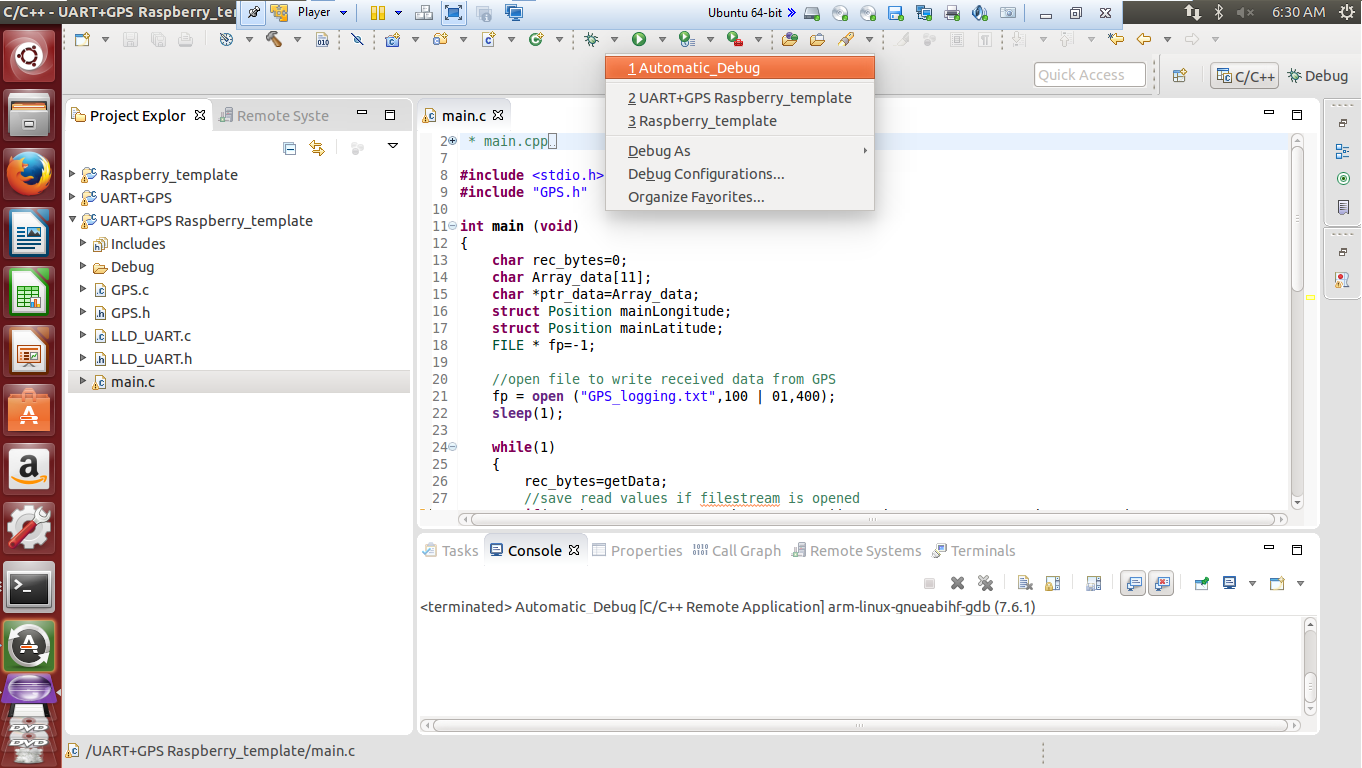
\includegraphics[width=0.9\textwidth]{fig/Dev_Concept/Debug8}
	\caption{Start Debugging}
	\label{fig:Debug8}
\end{figure}


%\subsection{Create project and start on the Raspberry}
%\label{subsubsec:subsubsec-eclipseproject}
%
%\workTodo{http://hertaville.com/2012/09/28/development-environment-raspberry-pi-cross-compiler/}







